\section{Theorie}
\label{sec:Theorie}

\subsection{Röntgenröhre}

Der schematische Aufbau einer Röntgenröhre ist in \autoref{fig:roehreAufbau} veranschaulicht.
Die emittierten Elektronen einer Heizkathode werden in einer evakuierten Röhre durch Anlegen einer Spannung $U$ in Richtung der Anode beschleunigt.
Der Potentialunterschied trägt hierbei samt der Elementarladung $e$ zur kinetischen Energie der auftreffenden Elektronen bei ($E_{kin} = e \cdot U$).
\begin{figure}
    \centering
    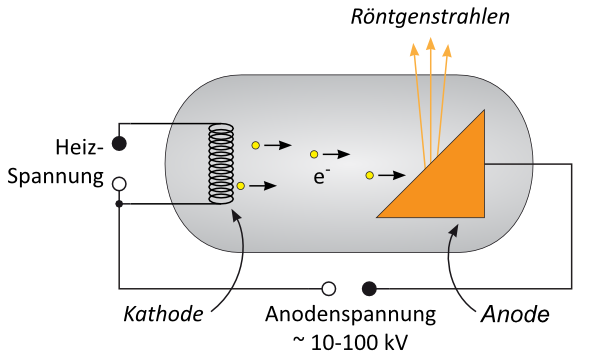
\includegraphics[width=0.5\linewidth]{abb/6621.png}
    \caption{Aufbau einer Röntgenröhre \cite{roehre}}
    \label{fig:roehreAufbau}
\end{figure}
Neben dem Großteil der Menge, die in Wärme umgewandelt wird, tritt durch entgegengerichteter Beschleunigung der geladenen Teilchen kontinuierliche Bremsstrahlung auf.
Ein weiterer nicht-kontinuierlicher Anteil des Spektrums einer Röntgenröhre (s. Abb. \ref{fig:roehreSpektrum}) ist die charakterisitsche Strahlung,
die starke Abhängigkeit des Anodenmaterials aufweist. Die durch einfallende Elektronen ionisierten Atome schlagen dabei ein weiteres Elektron aus der Hülle aus.
Das entstandende Loch schließt sich anschließend durch ein Elektron einer höheren Schale. Die Differenz der unterschiedlichen Energieniveaus wird dabei in Form eines Photons freigesetzt.
\begin{figure}
    \centering
    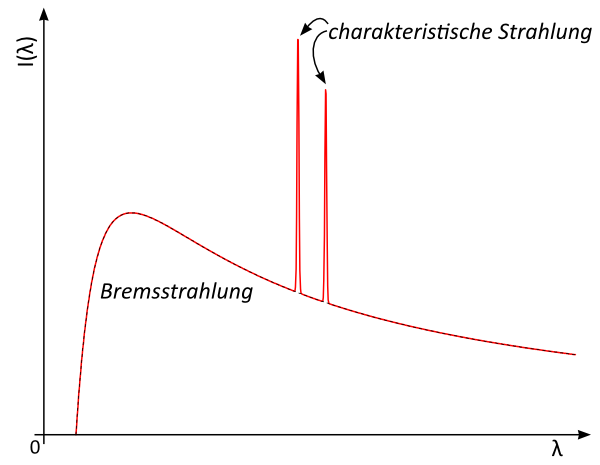
\includegraphics[width=0.5\linewidth]{abb/6635.png}
    \caption{Spektrum einer Röntgenröhre \cite{roehre}}
    \label{fig:roehreSpektrum}
\end{figure}

\subsection{Brechungsindex}
\subsubsection*{Grundlagen}
Aus dem Reflexionsgesetz, das besagt dass der Wellenvektor einer reflektierten Welle zum Lot der Grenzfläche den gleichen Winkel wie die einfallende Welle hat,
folgt durch die Stetigkeit an einer Grenzfläche
\begin{equation}
    k \sin \phi_1 = k' \sin \phi_2
    \label{eq:Stetigkeit}
\end{equation}
für eine gebrochene Welle.
Durch Umstellen lässt sich das Snellius'sche Brechnungsgesetz,
\begin{equation}
    \frac{\sin \phi_1}{\sin \phi_2} = \frac{c_1}{c_2} = \frac{\sqrt{\epsilon_2\mu_2}}{\sqrt{\epsilon_1\mu_1}} = \frac{n_2}{n_1} \text{,}
    \label{eq:Snellius}
\end{equation}
aufstellen. Hierbei wird der Brechungsindex definiert durch
\begin{equation}
    n := \sqrt{\epsilon\mu} = \frac{c_{Vakuum}}{c_{Materie}}.
\end{equation}
Neben des realen Brechungsindex $N$, der proportional zur Phasengeschwindigkeit ist,
wird ein Teil der elektromagnetischen Wellen durch die Materie, die sie durchwandert, absorbiert.
Demnachzufolge definiert man einen komplexen Brechungsindex
\begin{equation}
    N = n - i\kappa \text{.}
    \label{eq:nKomplex}
\end{equation}
Hierbei stellt $\kappa$ den Absorbtionskoeffizienten dar.

\subsubsection*{Röntgenstrahlung}
Im Röntgenspektrum von elektromagnetischen Wellen ist der Realteil des Brechungsindex wenig kleiner als 1 ($n = 1 - \delta$),
weil die Oszillationsfrequenz der äußeren Elektronen der bestrahlten Atome, die durch das elektrische Feld der Röntgenstrahlung zu Schwingungen oberhalb
ihrer Resonanzfrequenz gezwungen werden, geringer als die Schwingungsfrequenz des Röntgenbereiches ist.
Somit werden Röntgenstrahlen bei senkrechtem Auftreffen auf eine Grenzfläche im Gegensatz zu gewöhnlichem Licht vom Lot weg gebrochen.

\subsection{Fresnelsche Formeln}
Für eine quantitative Aussage über das Verhalten der Amplituden bei Reflexion und Brechung ist ein Fallunterschied der Polarisation der einfallenden Welle zur Einfallsebene zu berücksichtigen.
Jegliche andere Fälle kann man als Linearkombination dieser sehen.\cite{physik}
\subsubsection*{Senkrechte Polarisation}
Zwischen den Amplituden der reflektierten bzw. der gebrochenen und der einfallenden Welle besteht der Zusammenhang
\begin{equation}
    \left(\frac{E_{0,R}}{E_0}\right)_\perp = \frac{\frac{N_1}{\mu_1}\cos\phi_1 - \frac{N_2}{\mu_2}\cos\phi_2}{\frac{N_1}{\mu_1}\cos\phi_1 + \frac{N_2}{\mu_2}\cos\phi_2}
\end{equation}
und
\begin{equation}
    \left(\frac{E_{0,T}}{E_0}\right)_\perp = \frac{2\frac{N_1}{\mu_1}\cos\phi_1}{\frac{N_1}{\mu_1}\cos\phi_1 + \frac{N_2}{\mu_2}\cos\phi_2}\text{.}
\end{equation}
\subsubsection*{Parallele Polarisation}
Zwischen den Amplituden der reflektierten bzw. der gebrochenen und der einfallenden Welle besteht der Zusammenhang
\begin{equation}
    \left(\frac{E_{0,R}}{E_0}\right)_\parallel = -\frac{\frac{N_2}{\mu_2}\cos\phi_1 - \frac{N_1}{\mu_1}\cos\phi_2}{\frac{N_2}{\mu_2}\cos\phi_1 + \frac{N_1}{\mu_1}\cos\phi_2}
\end{equation}
und
\begin{equation}
    \left(\frac{E_{0,T}}{E_0}\right)_\parallel = -\frac{2\frac{N_1}{\mu_1}\cos\phi_1}{\frac{N_2}{\mu_2}\cos\phi_1 + \frac{N_1}{\mu_1}\cos\phi_2}\text{.}
\end{equation}
\subsubsection*{Röntgenstrahlung}
Mit $n_1 = 1$ und $n_2 < 1$ bei der Grenzfläche Luft-Materie ist $n_2 < n_1$ und somit sind ab einem bestimmten Winkel die Amplitudenverhältnisse komplex.\cite{nolting}
Dadurch unterziehen sich Röntgenstrahlen, die unter einem kritischen Winkel zum Lot auf der Grenzfläche treffen, bei Materieeinfall einer externen Totalreflexion.\cite{reflexion}
Dies ist gegeben, wenn $\phi_2 = \qty{90}{\degree}$ erreicht und somit $\sin\phi_2 = 1$. Der kritische Winkel kann mit \autoref{eq:Snellius} bestimmt werden durch
\begin{equation}
    \alpha_{krit} = \arcsin n_2 \text{.} \label{eq:krit}
\end{equation}

\subsection{Kiessig-Oszillationen}
Nach Überschreiten des Grenzwinkels $\phi_{krit}$ der Totalreflexion sind Maxima und Minima der reflektierten Intensität zu beobachten.
Diese Erscheinung ist ein Konstrukt der Interferenz der reflektierten Röntgenstrahlen an Oberfläche und Unterseite der Grenzflächenschicht (vgl. Abb. \ref{fig:kiessig}).
Durch die Lage der Minima und Maxima lassen sich mit den Ordnungszahlen $m$ und den Winkeln zweier Extremstellen sowohl die Dicke der Schichten als auch der Brechungsindex berechnen: \cite{kiessig}
\begin{align}
    d &= \frac{\lambda}{2}\sqrt{\frac{m_2²-m_1²}{\phi_2²-\phi_1²}} \\
    \delta &= \frac{1}{2}\frac{\phi_1² m_2² - \phi_2² m_1²}{m_2²-m_1²}
\end{align}

\begin{figure}
    \center
    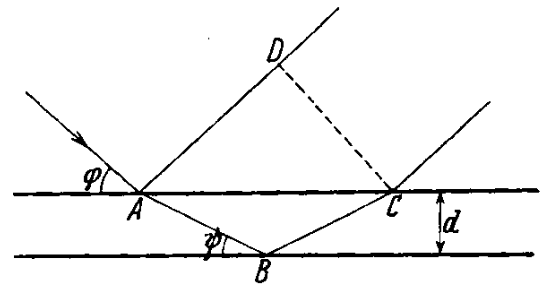
\includegraphics[width=0.6\linewidth]{abb/kiessig.png}
    \caption{Darstellung des Strahlenganges bei den Röntgeninterferenzen an dünnen Schichten \cite{kiessig}}
    \label{fig:kiessig}
\end{figure}

\subsection{Parratt-Algorithmus}
Der Parratt-Algorithmus beschäftigt sich mit der Form der Kurve von reflektierter Röntgenstrahlung gegenüber ihrem Glanzwinkel um die Materialbeschaffenheit der Spiegeloberfläche zu bestimmen.
Das Hauptaugenmerk ist dabei auf den Vergleich einer aufgenommenen Intensität mit der berechneten idealen Kurve oder vor und nach Anpassung des Materials.

